%%%% Header %%%%%%%%%%%%%%%%%%%%%%%%%%%%%%%%%%%%%%%%%%%%%%%%%%%%%%%%%%%%%%%%%%%

\documentclass[hyperref={bookmarks=false}]{beamer}

\usepackage{jobeam}

\bibliography{/home/jon/lucile/share/jowncloud/sci/refs/refs.bib}
\hyphenation{}

%%%% Meta Data %%%%%%%%%%%%%%%%%%%%%%%%%%%%%%%%%%%%%%%%%%%%%%%%%%%%%%%%%%%%%%%%

\title{
  Using Color in Data Visualization
}
\author{
  Jonas Schöley\texorpdfstring{\\\url{jschoeley@health.sdu.dk}}{}
}
\institute{
Max-Planck Odense Center on the Biodemography of Aging
}
\date{
  March 30, 2016
}

%%%% Titlepage %%%%%%%%%%%%%%%%%%%%%%%%%%%%%%%%%%%%%%%%%%%%%%%%%%%%%%%%%%%%%%%%

\begin{document}

%%%% Text %%%%%%%%%%%%%%%%%%%%%%%%%%%%%%%%%%%%%%%%%%%%%%%%%%%%%%%%%%%%%%%%%%%%%

\begin{frame}
\frametitle{Color-coding Magnitudes}

\center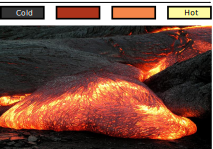
\includegraphics[width = 0.9\textwidth]{./fig/color_coded_luminance.pdf}

\blfootnote{Hawaii Volcano Observatory (2003). \url{http://hvo.wr.usgs.gov/multimedia/archive/2003/May/20030503-0021_DAS_large.jpg}}

\end{frame}

%%%%%%%%%%%%%%%%%%%%%%%%%%%%%%%%%%%%%%%%%%%%%%%%%%%%%%%%%%%%%%%%%%%%%%%%%%%%%%%

\begin{frame}
\frametitle{Color-coding Magnitudes}

\center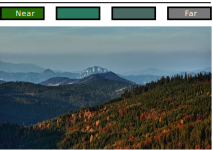
\includegraphics[width = 0.9\textwidth]{./fig/color_coded_saturation.pdf}

\blfootnote{Milan Cernak (2011). \enquote{Pieniny from Magura}.}

\end{frame}

%%%%%%%%%%%%%%%%%%%%%%%%%%%%%%%%%%%%%%%%%%%%%%%%%%%%%%%%%%%%%%%%%%%%%%%%%%%%%%%

\begin{frame}
\frametitle{Color-coding Categories}

\center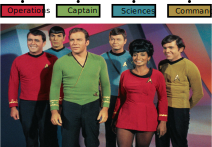
\includegraphics[width = 0.9\textwidth]{./fig/color_coded_hue.pdf}

\blfootnote{CBS Television.}

\end{frame}

%%%%%%%%%%%%%%%%%%%%%%%%%%%%%%%%%%%%%%%%%%%%%%%%%%%%%%%%%%%%%%%%%%%%%%%%%%%%%%%

\begin{frame}
\frametitle{Color-coding Data}

\center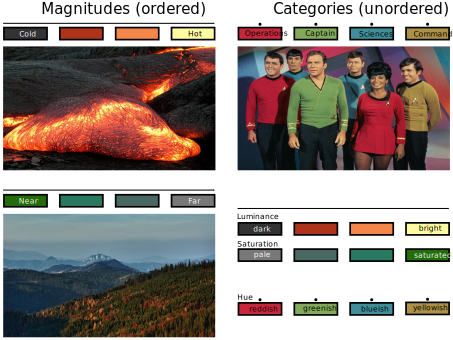
\includegraphics[width = \textwidth]{./fig/color_coded_complete.pdf}

\end{frame}

%%%%%%%%%%%%%%%%%%%%%%%%%%%%%%%%%%%%%%%%%%%%%%%%%%%%%%%%%%%%%%%%%%%%%%%%%%%%%%%

\begin{frame}
\frametitle{Color for Categorical Data}

\center\includegraphics[width = 0.9\textwidth]{./fig/gapminder_world_2013.pdf}

\blfootnote{Gapminder World (2014). \url{http://www.gapminder.org/downloads/gapminder-world-poster-2013/}}

\end{frame}

%%%%%%%%%%%%%%%%%%%%%%%%%%%%%%%%%%%%%%%%%%%%%%%%%%%%%%%%%%%%%%%%%%%%%%%%%%%%%%%

\begin{frame}
\frametitle{Ineffective Color-coding}

\center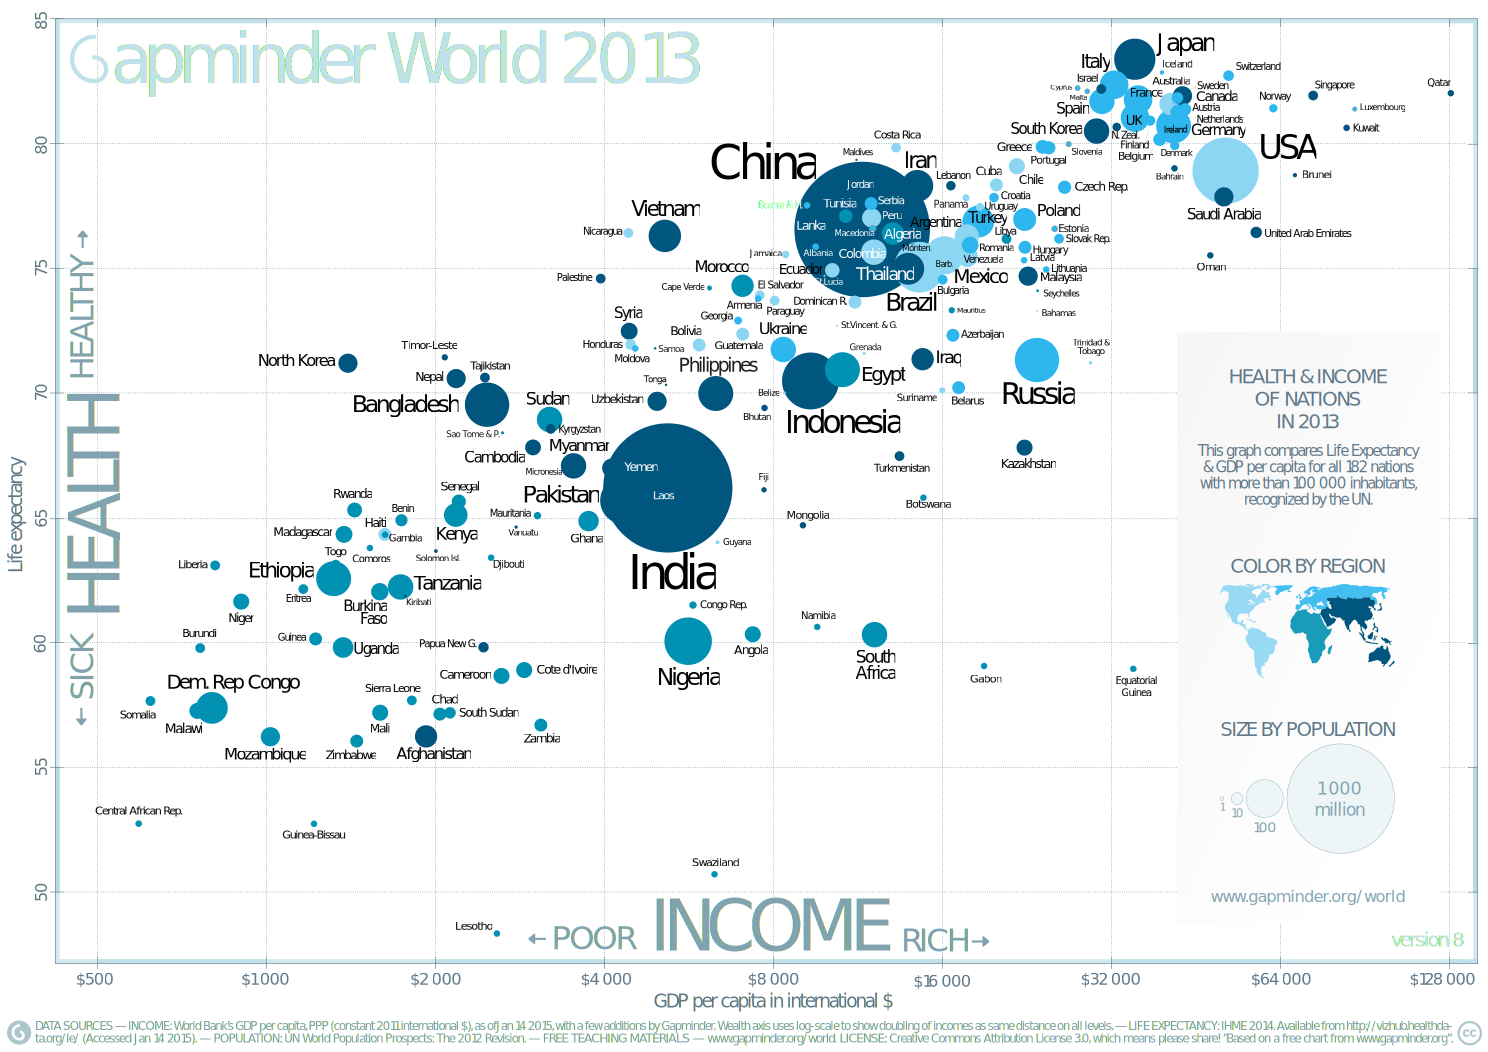
\includegraphics[width = 0.9\textwidth]{./fig/gapminder_world_2013_mono.pdf}

\blfootnote{Redrawn from Gapminder World (2014).}

\end{frame}

%%%%%%%%%%%%%%%%%%%%%%%%%%%%%%%%%%%%%%%%%%%%%%%%%%%%%%%%%%%%%%%%%%%%%%%%%%%%%%%

\begin{frame}
\frametitle{Pick Meaningful Colors}

\center\includegraphics[width = 0.6\textwidth]{./fig/lin_etal-2013-figure1c.png}\\
\center\includegraphics[width = 0.6\textwidth]{./fig/lin_etal-2013-figure1a.png}

\blfootnote{\fullcite{Lin2013}.}

\end{frame}

%%%%%%%%%%%%%%%%%%%%%%%%%%%%%%%%%%%%%%%%%%%%%%%%%%%%%%%%%%%%%%%%%%%%%%%%%%%%%%%

\begin{frame}
\frametitle{How Would You Color Death?}

\center\includegraphics[width = 0.47\textwidth]{./fig/codus2014_150dpi.png}

\blfootnote{Jonas Schöley (2016). \url{github.com/jschoeley/codus2014}}

\end{frame}

%%%%%%%%%%%%%%%%%%%%%%%%%%%%%%%%%%%%%%%%%%%%%%%%%%%%%%%%%%%%%%%%%%%%%%%%%%%%%%%

\begin{frame}
\frametitle{Color for Metric Data}

\center\includegraphics[width = 0.9\textwidth]{./fig/malaria.jpg}

\blfootnote{Cutout from Francis Walker (1874). \enquote{Statistical Atlas of the United States}. \url{https://www.loc.gov/item/05019329/}}

\end{frame}

%%%%%%%%%%%%%%%%%%%%%%%%%%%%%%%%%%%%%%%%%%%%%%%%%%%%%%%%%%%%%%%%%%%%%%%%%%%%%%%

\begin{frame}
\frametitle{Ineffective Color-coding}

\center\includegraphics[width = 0.9\textwidth]{./fig/elevation.png}

\blfootnote{South East Maps \& Aerial Photographic Systems. \url{http://www.clemson.edu/ces/geolk12/semaps/seregional/hires/digielmap.jpg}}

\end{frame}

%%%%%%%%%%%%%%%%%%%%%%%%%%%%%%%%%%%%%%%%%%%%%%%%%%%%%%%%%%%%%%%%%%%%%%%%%%%%%%%

\begin{frame}
\frametitle{Discrete vs. Continuous Color Scales}

\center\includegraphics[width = 0.65\textwidth]{./fig/discrete.png}\\
\center\includegraphics[width = 0.65\textwidth]{./fig/cont.png}

\blfootnote{Jonas Schöley (2016). \enquote{The Human Mortality Explorer}. \url{jschoeley.shinyapps.io/hmdexp}}

\end{frame}

%%%%%%%%%%%%%%%%%%%%%%%%%%%%%%%%%%%%%%%%%%%%%%%%%%%%%%%%%%%%%%%%%%%%%%%%%%%%%%%

\begin{frame}
\frametitle{Color for Divergent Data}

\center\includegraphics[width = 0.8\textwidth]{./fig/divergent.png}

\blfootnote{Jonas Schöley (2016). \enquote{The Human Mortality Explorer}. \url{jschoeley.shinyapps.io/hmdexp}}

\end{frame}

%%%%%%%%%%%%%%%%%%%%%%%%%%%%%%%%%%%%%%%%%%%%%%%%%%%%%%%%%%%%%%%%%%%%%%%%%%%%%%%

\begin{frame}
\frametitle{Separating Foreground \& Background}

\center\includegraphics[width = 0.6\textwidth]{./fig/picasso.jpg}

\blfootnote{Pablo Picasso (1905). \enquote{Au Lapin Agile}.}

\end{frame}

%%%%%%%%%%%%%%%%%%%%%%%%%%%%%%%%%%%%%%%%%%%%%%%%%%%%%%%%%%%%%%%%%%%%%%%%%%%%%%%

\begin{frame}
\frametitle{Separating Foreground \& Background}

\center\includegraphics[width = 0.62\textwidth]{./fig/fb0.pdf}

\blfootnote{Data: \url{gapminder.org} -- displayed are data for the year 2007.}

\end{frame}

%%%%%%%%%%%%%%%%%%%%%%%%%%%%%%%%%%%%%%%%%%%%%%%%%%%%%%%%%%%%%%%%%%%%%%%%%%%%%%%

\begin{frame}
\frametitle{Separating Foreground \& Background}

\center\includegraphics[width = 0.62\textwidth]{./fig/fb1.pdf}

\blfootnote{Data: \url{gapminder.org}}

\end{frame}

%%%%%%%%%%%%%%%%%%%%%%%%%%%%%%%%%%%%%%%%%%%%%%%%%%%%%%%%%%%%%%%%%%%%%%%%%%%%%%%

\begin{frame}
\frametitle{Separating Foreground \& Background}

\center\includegraphics[width = 0.62\textwidth]{./fig/fb2.pdf}

\blfootnote{Data: \url{gapminder.org}}

\end{frame}

%%%%%%%%%%%%%%%%%%%%%%%%%%%%%%%%%%%%%%%%%%%%%%%%%%%%%%%%%%%%%%%%%%%%%%%%%%%%%%%

\begin{frame}
\frametitle{Separating Foreground \& Background}

\center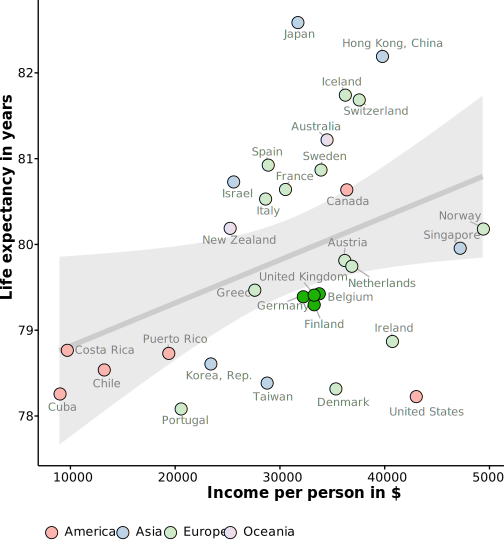
\includegraphics[width = 0.62\textwidth]{./fig/fb3.pdf}

\blfootnote{Data: \url{gapminder.org}}

\end{frame}

%%%%%%%%%%%%%%%%%%%%%%%%%%%%%%%%%%%%%%%%%%%%%%%%%%%%%%%%%%%%%%%%%%%%%%%%%%%%%%%

\begin{frame}
\frametitle{You Take Control!}

\center\includegraphics[width = \textwidth]{./fig/color_picker.png}

\end{frame}

%%%%%%%%%%%%%%%%%%%%%%%%%%%%%%%%%%%%%%%%%%%%%%%%%%%%%%%%%%%%%%%%%%%%%%%%%%%%%%%

\end{document}